\documentclass{article}
\usepackage{spikey}
\usepackage{amsmath}
\usepackage{mathrsfs}
\usepackage{amssymb}
\usepackage{soul}
\usepackage{float}
\usepackage{graphicx}
\usepackage{hyperref}
\usepackage{fancyhdr}
%\usepackage{xcolor}
\usepackage{chngcntr}
\usepackage{centernot}
\usepackage[shortlabels]{enumitem}
\usepackage[margin=1truein]{geometry}
\usepackage{tkz-graph}
\usepackage{dsfont}
\usepackage{caption}
\usepackage{subcaption}
\usepackage{booktabs}
\usepackage[yyyymmdd,hhmmss]{datetime}

\usepackage{tikz}
\usetikzlibrary{arrows}

\usepackage{setspace}
\linespread{1.15}
\usepackage[margin=1truein]{geometry}

\counterwithin{equation}{section}
\counterwithin{figure}{section}

\usepackage{listings}
 
\definecolor{codegreen}{rgb}{0,0.6,0}
\definecolor{codegray}{rgb}{0.5,0.5,0.5}
\definecolor{codeblue}{rgb}{0.3,0.5,0.8}
\definecolor{codepurple}{rgb}{0.58,0,0.82}
%\definecolor{backcolour}{rgb}{0.95,0.95,0.92}
\definecolor{backcolour}{rgb}{1,1,1}

\lstdefinestyle{mystyle}{
    backgroundcolor=\color{backcolour},   
    commentstyle=\color{codegreen},
    keywordstyle=\color{magenta},
    numberstyle=\tiny\color{codegray},
    stringstyle=\color{codepurple},
    basicstyle=\ttfamily\footnotesize,
    breakatwhitespace=false,         
    breaklines=true,                 
    captionpos=b,                    
    keepspaces=true,                 
    numbers=left,                    
    numbersep=5pt,                  
    showspaces=false,                
    showstringspaces=false,
    showtabs=false,                  
    tabsize=4
}

\lstset{style=mystyle}

\title{CSC413: Programming Assignment 4}
\date{\today\ at \currenttime}
\author{Tianyu Du (1003801647)}
\begin{document}
	\maketitle
	\section{Part 1: Deep Convolutional GAN (DCGAN) [4pt]}
	\subsection{Generator}
	\textbf{Implementation} Please note that I modified the \texttt{forward} method a little bit as well.
	\begin{lstlisting}[language=python]
class DCGenerator(nn.Module):
    def __init__(self, noise_size, conv_dim, spectral_norm=False):
        super(DCGenerator, self).__init__()

        self.conv_dim = conv_dim # 32

        ###########################################
        ##   FILL THIS IN: CREATE ARCHITECTURE   ##
        ###########################################

        self.linear_bn = nn.Linear(100, self.conv_dim*4*4*4) # (100, 2048)
        self.upconv1 = upconv(self.conv_dim*4, self.conv_dim*2, 5, stride=2, padding=2, batch_norm=True, spectral_norm=spectral_norm)
        self.upconv2 = upconv(self.conv_dim*2, self.conv_dim, 5, stride=2, padding=2, batch_norm=True, spectral_norm=spectral_norm)
        self.upconv3 = upconv(self.conv_dim, 3, 5, stride=2, padding=2, batch_norm=True, spectral_norm=spectral_norm)

    def forward(self, z):
        """Generates an image given a sample of random noise.

            Input
            -----
                z: BS x noise_size x 1 x 1   -->  BSx100x1x1 (during training)

            Output
            ------
                out: BS x channels x image_width x image_height  -->  BSx3x32x32 (during training)
        """
        batch_size = z.size(0)
        # Extra reshape
        z = z.view(batch_size, -1)
        out = F.relu(self.linear_bn(z)).view(-1, self.conv_dim*4, 4, 4)    # BS x 128 x 4 x 4
        out = F.relu(self.upconv1(out))  # BS x 64 x 8 x 8
        out = F.relu(self.upconv2(out))  # BS x 32 x 16 x 16
        out = F.tanh(self.upconv3(out))  # BS x 3 x 32 x 32
        
        out_size = out.size()
        if out_size != torch.Size([batch_size, 3, 32, 32]):
            raise ValueError("expect {} x 3 x 32 x 32, but get {}".format(batch_size, out_size))
        return out

	\end{lstlisting}
	\subsection{Training Loop}
	\textbf{Implementation}
	\begin{lstlisting}[language=python]
def gan_training_loop(dataloader, test_dataloader, opts):
    """Runs the training loop.
        * Saves checkpoint every opts.checkpoint_every iterations
        * Saves generated samples every opts.sample_every iterations
    """

    # Create generators and discriminators
    G, D = create_model(opts)

    g_params = G.parameters()  # Get generator parameters
    d_params = D.parameters()  # Get discriminator parameters

    # Create optimizers for the generators and discriminators
    g_optimizer = optim.Adam(g_params, opts.lr, [opts.beta1, opts.beta2])
    d_optimizer = optim.Adam(d_params, opts.lr * 2., [opts.beta1, opts.beta2])

    train_iter = iter(dataloader)

    test_iter = iter(test_dataloader)

    # Get some fixed data from domains X and Y for sampling. These are images that are held
    # constant throughout training, that allow us to inspect the model's performance.
    fixed_noise = sample_noise(100, opts.noise_size)  # # 100 x noise_size x 1 x 1

    iter_per_epoch = len(train_iter)
    total_train_iters = opts.train_iters

    losses = {"iteration": [], "D_fake_loss": [], "D_real_loss": [], "G_loss": []}

    gp_weight = 10

    try:
        for iteration in range(1, opts.train_iters + 1):

            # Reset data_iter for each epoch
            if iteration % iter_per_epoch == 0:
                train_iter = iter(dataloader)

            real_images, real_labels = train_iter.next()
            real_images, real_labels = to_var(real_images), to_var(real_labels).long().squeeze()

            # ones = Variable(torch.Tensor(real_images.shape[0]).float().cuda().fill_(1.0), requires_grad=False)

            for d_i in range(opts.d_train_iters):
                d_optimizer.zero_grad()

                # FILL THIS IN
                # 1. Compute the discriminator loss on real images
                D_real_loss = torch.mean((D(real_images) - 1) ** 2) / 2

                # 2. Sample noise
                noise = torch.randn_like(fixed_noise)

                # 3. Generate fake images from the noise
                fake_images = G(noise)
                
                # 4. Compute the discriminator loss on the fake images
                D_fake_loss = torch.mean(D(fake_images) ** 2) / 2

                # ---- Gradient Penalty ----
                if opts.gradient_penalty:
                    alpha = torch.rand(real_images.shape[0], 1, 1, 1)
                    alpha = alpha.expand_as(real_images).cuda()
                    interp_images = Variable(alpha * real_images.data + alpha * fake_images.data, requires_grad=True).cuda()
                    D_interp_output = D(interp_images)

                    gradients = torch.autograd.grad(outputs=D_interp_output, inputs=interp_images,
                                                    grad_outputs=torch.ones(D_interp_output.size()).cuda(),
                                                    create_graph=True, retain_graph=True)[0]
                    gradients = gradients.view(real_images.shape[0], -1)
                    gradients_norm = torch.sqrt(torch.sum(gradients ** 2, dim=1) + 1e-12)

                    gp = gp_weight * gradients_norm.mean()
                else:
                    gp = 0.0

                # --------------------------
                # 5. Compute the total discriminator loss
                D_total_loss = D_real_loss + D_fake_loss

                D_total_loss.backward()
                d_optimizer.step()

            ###########################################
            ###          TRAIN THE GENERATOR        ###
            ###########################################

            g_optimizer.zero_grad()

            # FILL THIS IN
            # 1. Sample noise
            noise = torch.randn_like(fixed_noise)

            # 2. Generate fake images from the noise
            fake_images = G(noise)

            # 3. Compute the generator loss
            G_loss = torch.mean((D(fake_images) - 1)**2)

            G_loss.backward()
            g_optimizer.step()

            # Print the log info
            if iteration % opts.log_step == 0:
                losses['iteration'].append(iteration)
                losses['D_real_loss'].append(D_real_loss.item())
                losses['D_fake_loss'].append(D_fake_loss.item())
                losses['G_loss'].append(G_loss.item())
                print('Iteration [{:4d}/{:4d}] | D_real_loss: {:6.4f} | D_fake_loss: {:6.4f} | G_loss: {:6.4f}'.format(
                    iteration, total_train_iters, D_real_loss.item(), D_fake_loss.item(), G_loss.item()))

            # Save the generated samples
            if iteration % opts.sample_every == 0:
                gan_save_samples(G, fixed_noise, iteration, opts)

            # Save the model parameters
            if iteration % opts.checkpoint_every == 0:
                gan_checkpoint(iteration, G, D, opts)

    except KeyboardInterrupt:
        print('Exiting early from training.')
        return G, D

    plt.figure()
    plt.plot(losses['iteration'], losses['D_real_loss'], label='D_real')
    plt.plot(losses['iteration'], losses['D_fake_loss'], label='D_fake')
    plt.plot(losses['iteration'], losses['G_loss'], label='G')
    plt.legend()
    plt.savefig(os.path.join(opts.sample_dir, 'losses.png'))
    plt.close()
    return G, D
	\end{lstlisting}
	\subsection{Experiments}
	
	\section{Part 3: BigGAN [2pt]}
	\subsection{BigGAN Experiments}
	\subsubsection{Question 1}
	\paragraph{Method} Given two classes with embeddings $\mathbf{r}_{class1}$ and $\mathbf{r}_{class2}$ in T-SNE space, to decide whether they are good candidate for linear interpolation, I looked at convex combinations of two classes' embeddings in figure \ref{tsne}.
	Let $\Phi$ denote the set of convex combinations:
	\begin{align}
		\Phi = \{\alpha \mathbf{r}_{c l a s s 1}+(1-\alpha) \mathbf{r}_{c l a s s 2}: \alpha \in[0,1]\}
	\end{align}
	Linear interpolations between these two classes are basically taking points in set $\Phi$ and visualizing them.
	If there are many \ul{other classes' embeddings} on or near the set $\Phi$, points in $\Phi$ are likely to be associated with meaningful visualizations.
	Therefore, linear interpolations between these two classes are likely to generate meaningful results.
	Otherwise, these two classes are not good candidates for linear interpolation.
	\begin{figure}[H]
		\caption{T-SNE Plot}
		\centering
		\label{tsne}
		\medbreak
		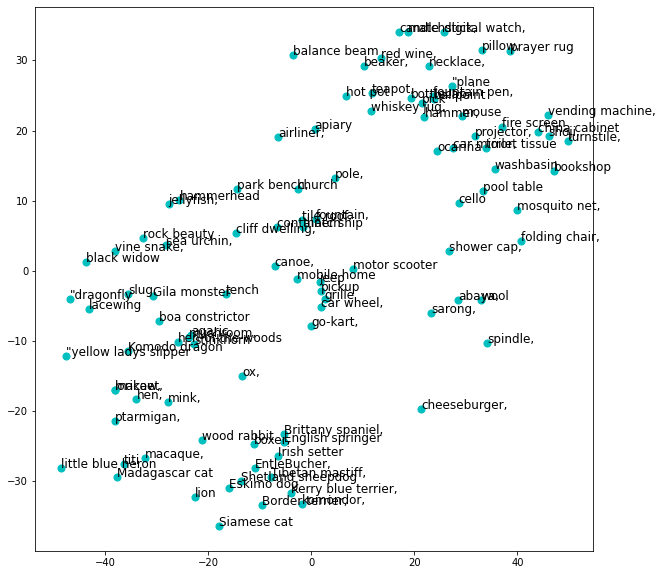
\includegraphics[width=0.7\linewidth]{./tsne.png}
	\end{figure}
	\paragraph{Good Candidate Match 1} There are many classes near the segment between \texttt{folding chair} and \texttt{vending machine} (right-up corner), so linear interpolation should be meaningful.
%	\begin{figure}[H]
%		\caption{Folding Chair and Vending Machine}
%		\centering
%		\medbreak
%		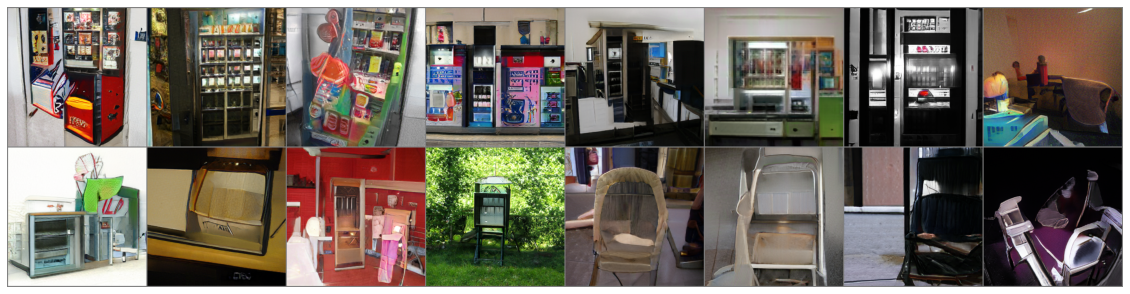
\includegraphics[width=0.7\linewidth]{./foldingchair_vendingmachine.png}
%	\end{figure}
	
	\paragraph{Good Candidate Match 2} Similarly, there are many classes on the line between \texttt{bookshop} and \texttt{hot pot} (right-up corner), so they are ideal for linear interpolation.

%	\begin{figure}[H]
%		\caption{Hot Pot and Bookshop}
%		\centering
%		\medbreak
%		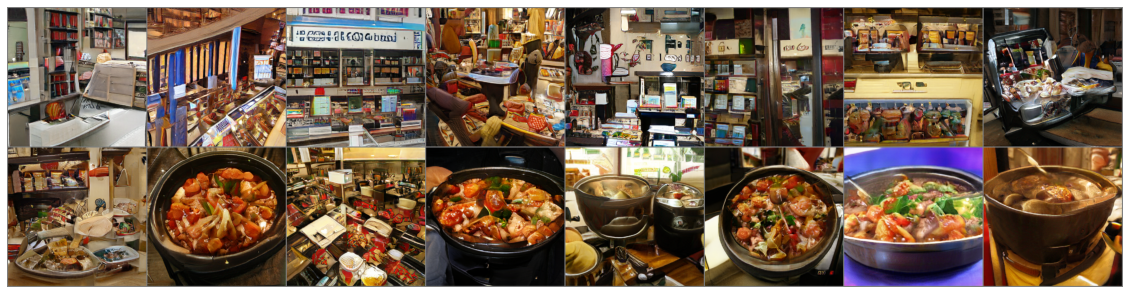
\includegraphics[width=0.7\linewidth]{./hotpot_bookshop.png}
%	\end{figure}
	
	\paragraph{Bad Candidate Match 1} There are no other classes' embeddings are in between embeddings of \texttt{Go-Kart} and \texttt{Chessburger} in T-SNE plot, so they are not good match.
%	\begin{figure}[H]
%		\caption{Go-Kart and Chessburger}
%		\centering
%		\medbreak
%		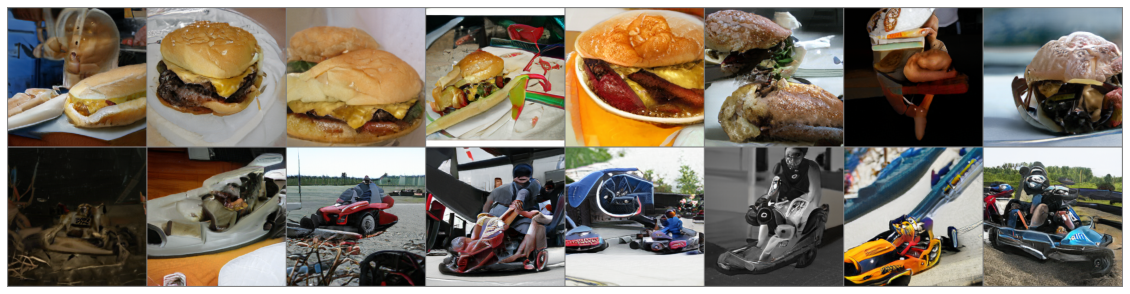
\includegraphics[width=0.7\linewidth]{./gokart_cheeseburger.png}
%	\end{figure}

	\paragraph{Bad Candidate Pair 2} Similarly, \texttt{Ox} and \texttt{Chessburger} are not good match.
%	\begin{figure}[H]
%		\caption{Ox and Chessburger}
%		\centering
%		\medbreak
%		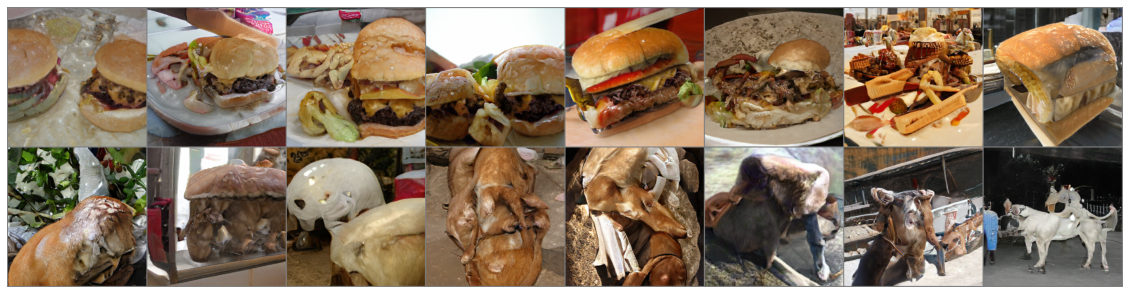
\includegraphics[width=0.7\linewidth]{./ox_chessburger.png}
%	\end{figure}

	\subsubsection{Question 2}
	\textbf{Implementation}
	\begin{lstlisting}[language=python]
#Linear interpolation between two class embedings
def generate_linear_interpolate_sample(G, batch_size, class_label1, class_label2, alpha):
  	G.eval()
  	G.to(DEVICE)
  	with torch.no_grad():
	    z = torch.randn(batch_size, G.dim_z).to(DEVICE)
	    class1_emb = G.shared(torch.tensor(class_label1).to(DEVICE)*torch.ones((batch_size,)).to(DEVICE).long())
	    class2_emb = G.shared(torch.tensor(class_label2).to(DEVICE)*torch.ones((batch_size,)).to(DEVICE).long())
	
	    ###########################################
	    ##   FILL THIS IN: CREATE NEW EMBEDDING  ##
	    ###########################################    
	    new_emb = alpha * class1_emb + (1 - alpha) * class2_emb
	
	    images = G(z, new_emb)
  	return images
	\end{lstlisting}
	\textbf{Linear Interpolation Results}
	\begin{figure}[H]
		\caption{Good Match 1: Folding Chair and Vending Machine}
		\centering
		\medbreak
		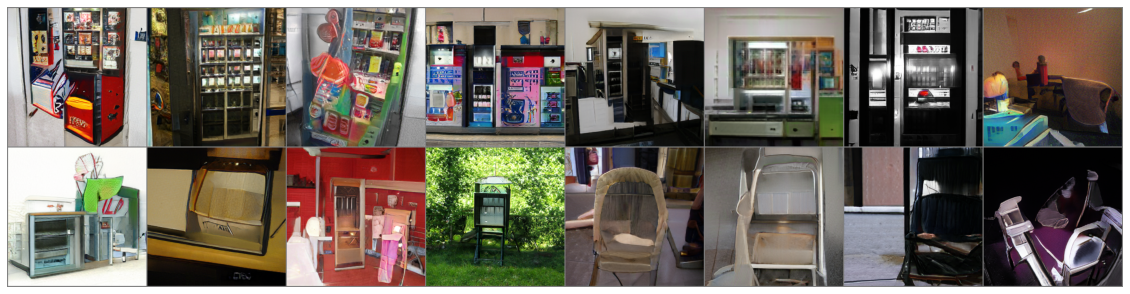
\includegraphics[width=0.7\linewidth]{./foldingchair_vendingmachine.png}
	\end{figure}

	\begin{figure}[H]
		\caption{Good Match 2 Hot Pot and Bookshop}
		\centering
		\medbreak
		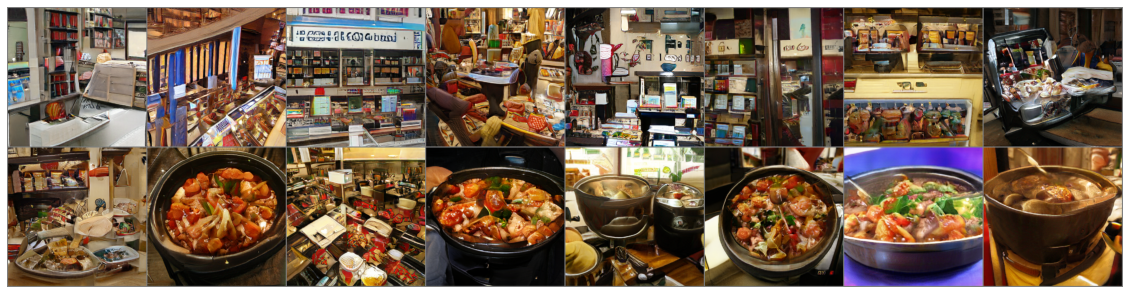
\includegraphics[width=0.7\linewidth]{./hotpot_bookshop.png}
	\end{figure}
	
	\begin{figure}[H]
		\caption{Bad Match 1 Go-Kart and Chessburger}
		\centering
		\medbreak
		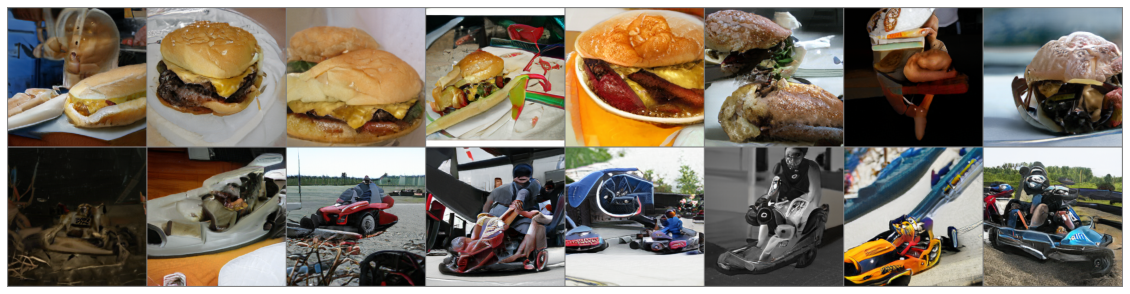
\includegraphics[width=0.7\linewidth]{./gokart_cheeseburger.png}
	\end{figure}

	\begin{figure}[H]
		\caption{Bad Match 2 Ox and Chessburger}
		\centering
		\medbreak
		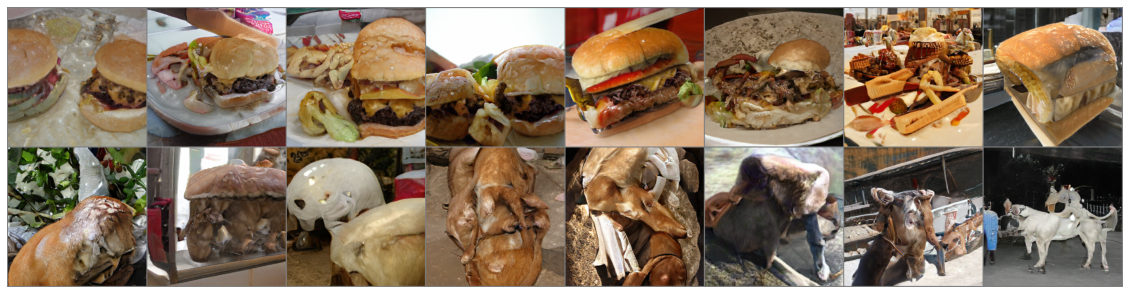
\includegraphics[width=0.7\linewidth]{./ox_chessburger.png}
	\end{figure}
\end{document}

































